\documentclass[parskip=half, a4paper,twoside,final]{article}
%----Eingebundene Bibliotheken-----
\usepackage[ngerman]{babel}         % Deutsches Sprachpaket
\usepackage[utf8]{inputenc}         % Eingaben codieren
\usepackage[T1]{fontenc}            % Umlaute codieren, Silbentrennung
\usepackage{amsmath, amssymb}       % Mathe
\usepackage{amsthm,amstext,amsxtra} % Symbole für Mathe
\usepackage{mathtools}              % \Aboxed Boxen in align
\usepackage{wrapfig}                % Bilder umfließen
\usepackage{svg}                    % Vektorgraphiken einbinden
\usepackage{geometry}               % Papierformat
\usepackage{tabularx}               % Tabellen
\usepackage{xcolor,colortbl}        % Farben
\usepackage{graphicx}               % Für Limes Definition wichtig
\usepackage{soul}                   % Unterstreichungen
\usepackage[section]{placeins}      % \Floatbarrier
\usepackage{wrapfig}                % Bilder umfließen
\usepackage{enumerate}              % Aufzählungen
\usepackage{footnote}               % Fußzeilen
\usepackage{booktabs}               % publication quality tables
\usepackage[hyphens]{url}           % \url{}
\usepackage{bm}                     % bold symbols \bm{r}
\usepackage{dsfont}                 % identity matrix \mathds{1}
\usepackage{enumitem}               % itemize Umgebungen customizen
\usepackage{esint}                  % Doppelintegrale
\usepackage{fancyhdr}               % schöne Kopf- und Fußzeilen
\usepackage{lmodern}
\usepackage{tikz}
\usepackage{pgfmath, pgfplots}
\usepackage[labelfont=bf]{subcaption}
\usepackage[square,numbers,sort&compress]{natbib}
\usepackage{mhchem}                 % Chemistry Package
\usepackage{physics}
\usepackage{chemfig}
\usepackage[detect-all,
            locale=DE,binary-units,
            exponent-product=\cdot
            ]{siunitx}              % \SI{12}{\gram}
%siunitx stellt für Tabellen den Spaltentyp S bereit ==> Ausrichtung an Dezimaltrennzeichen
\usepackage[position=below,
            tableposition=top,
            format=hang,
            labelfont=it,
            labelfont=bf,
            ]{caption}              % Settings für Captions
\captionsetup[wrapfigure]{name=Abb.}
\usepackage[europeanvoltages,
            europeancurrents,
            europeanresistors,
            americaninductors,
            europeanports
            ]{circuitikz}           % Schaltungen
\usepackage{chngcntr}               % vor hyperref laden!
  \counterwithin*{equation}{section}
  \counterwithin*{figure}{section}
  \counterwithin*{table}{section}

\usepackage[final,
            pdfauthor={Martin Beyer, Vanessa Huth},
            pdfsubject={Fortgeschrittenen-Praktikum},
            pdffitwindow=true,      % resize document window
            pdftitle={Fortgeschrittenen-Praktikum},
            bookmarks=true,         % lesezeichen-Liste
            bookmarksopen=true,     % Lesezeichen geöffnet
            bookmarksopenlevel=1,
            bookmarksnumbered=true,
            colorlinks=true,        % fuer Druckversion auf "false"
            linkcolor=blue,         % Table of Contents, Footnotes
            urlcolor=blue,          % fuer eingebunden URLs
            citecolor=blue,         % Equations, References
            filecolor=blue,
            pdfborder={0 0 0},      % keine Rahmen um Links: {0 0 0}
            ]{hyperref}


% Commands
\renewcommand{\sfdefault}{lmss}     % latin modern sans serif
\newcommand{\R}{\mathbb{R}}         % Reelle Zahlen
\newcommand{\N}{\mathbb{N}}         % Natürliche Zahlen
\newcommand{\C}{\mathbb{C}}         % Komplexe Zahlen
\newcommand{\de}{\mathrm{d}}      % Differential
\newcommand{\entspricht}{\mathrel{\widehat{=}}}

\DeclareSIUnit{\eV}{\text{eV}}
\DeclareSIUnit{\voltpeakpeak}{\volt{\textsubscript{pp}}}

% Dokumenteneinstellungen
\setlength{\parindent}{0px}         % remove indent in new paragraph
\setlength{\parindent}{0px}         % keine Absätze durch Leerzeilen im Code
\emergencystretch=1em % Definiert den Leerraum, der innerhalb einer Zeile zusätzlich verteilt werden darf.
\setlength{\topmargin}{-5mm} % 210mm = 8.2677165in
\newlength{\mylength}
\setlength{\mylength}{\paperwidth}
\addtolength{\mylength}{-2in} % standardmäßig wird den Seitenrändern jeweils noch 1in = 25.4mm hinzuaddiert
\setlength{\textwidth}{145mm}
\setlength{\textheight}{230mm}
\addtolength{\mylength}{-\textwidth}
\setlength{\oddsidemargin}{10mm}
\addtolength{\mylength}{-\oddsidemargin}
\setlength{\evensidemargin}{\mylength}
\setlength{\marginparwidth}{1.7cm}
\interfootnotelinepenalty=10000

% Umdefinition von \textcolor ********************************************************
\makeatletter
\renewcommand*{\@textcolor}[3]{%
	\protect\leavevmode
	\begingroup
	\color#1{#2}#3%
	\endgroup
}
\makeatother
% Damit das auch im Mathemodus anwendbar ist und dort z.B. die Leerzeichen nicht wie im Textmodus gesetzt werden.

\pgfplotsset
{compat=newest, % aktuelle Version: 1.16 [29.05.2018]
	/pgf/number format/.cd, % cd steht fuer current directory
	%  	use comma, % Komma als Dezimaltrennzeichen %%% UNCOMMENT THIS !!!
	1000 sep={} % Legt das Tausendertrennzeichen fest
}
%\usepgfplotslibrary{external} % Section 7.1.1 Using the Automatic Externalization Framework of TikZ
%\tikzexternalize[prefix=FiguresTikZ/] % activate externalization! Use subdirectory [FiguresTikZ]
\usepgfplotslibrary{fillbetween}
\usepgfplotslibrary{polar}
\usetikzlibrary{arrows.meta}
\usetikzlibrary{calc}
\usetikzlibrary{datavisualization.formats.functions}
\usetikzlibrary{intersections}
\usetikzlibrary{patterns}
\usetikzlibrary{pgfplots.colormaps}
\usetikzlibrary{plotmarks}
\usetikzlibrary{shapes.geometric}

% Generelle Festlegung des Styles fuer Blockschemata (Plaene fuer Regelkreise, etc.)
\tikzstyle{block} = [draw, fill=blue!20, rectangle, minimum height=1cm, minimum width=1cm]%, minimum width=6em]
\tikzstyle{sum} = [draw, fill=blue!20, circle, node distance=1cm]
\tikzstyle{input} = [coordinate]
\tikzstyle{output} = [coordinate]
\tikzstyle{pinstyle} = [pin edge={to-,thin,black}]

\DeclareSIUnit{\calorie}{cal}

\begin{document}
\setlength{\marginparsep}{2em}
\renewcommand{\theequation}{\arabic{section}.\arabic{equation}}
\renewcommand{\thefigure}{\arabic{section}.\arabic{figure}}
\renewcommand{\thetable}{\arabic{section}.\arabic{table}}

% Anfang ********************************************************
\begin{center}
\thispagestyle{empty}
  
\includegraphics[width=0.75\textwidth]{../UniJena_BildWortMarke_black.pdf}\\[4em]
  \Large
  Ausarbeitung zum Versuch\\[2em]
  \Huge
  Festkörpereigenschaften bei tiefen Temperaturen\\
  \vspace{2cm}
  \Large
  Martin Beyer und Vanessa Huth\\[2em]
  Abgabe: 30. September 2020\\[2em]
  Betreuer: Matthias Thürk\\[5em]
  \begin{flushleft}
  	Bewertung und Ausarbeitung:\\[2em]
		Protokollführung und Form:\\[1em]
		Ergebnisse, Auswertung und Interpretation:\\[1em]
		Bemerkungen und Hinweise des Betreuers:
  \end{flushleft}
\end{center}
\clearpage

\pagestyle{fancy}
\renewcommand{\headrulewidth}{0pt}
\renewcommand{\footrulewidth}{0.5pt}
\renewcommand{\sectionmark}[1]{\markright{#1}}
\fancyhead[RO,LE]{\textbf{Tieftemperatur}}
\fancyhead[RE,LO]{\rightmark}
\fancyfoot[LE,RO]{\bfseries\thepage}
\fancyfoot[CO,CE]{Protokoll}
\renewcommand{\headrulewidth}{0.5pt}
\renewcommand{\footrulewidth}{0.5pt}

\setcounter{equation}{0}
\setcounter{figure}{0}

% *********************************************
% ***** KAPITEL 1 *****************************
% *********************************************
\tableofcontents
% \pagenumbering{gobble}% remove page numbering
\newpage
% \pagenumbering{arabic}
\section{Aufgabenstellung} \label{sec:Aufgabenstellung}

\subsection{Aufbau geeigneter Tieftemperaturmesstechnik}

Es werden Widerstandsthermometer Pt 100 und Pt 1000, sowie Siliziumdioden als Sekundärthermometer verwendet. Es soll die Anfangstemperatur an den Sensoren auf folgende Weisen vermessen werden:
\begin{enumerate}
  \item Zweileiterschaltung mit Temperaturmessfunktion des Digitalvoltmeters (DVM), einmal ohne und einmal mit Kompensation des Messleitungswiderstandes.
  \item Zweileiterschaltung mit Konstantstromquelle und Spannungsmessung mit DVM.
  \item Vierleiterschaltung mit Konstantstromquelle und Spannungsmessung mit DVM.
\end{enumerate}

Es werden die Vor- und Nachteile der betrachteten Verfahren diskutiert.

\subsection{Temperaturabhängiger Widerstandes eines Halbleiters}

\begin{enumerate}
  \item Es wird eine Messchaltung zur Bestimmung des temperaturabhängigen Widerstandes und der Temperatur eines Gold-dotierten Germaniumhalbleiters aufgebaut.
  \item Der Abkühlvorgang der Gifford-McMahon Kleinkältemaschine wird aufgenommen.
  \item Es erfolgt eine Bestimmung der wirksamen Bandlücke zwischen Akzeptorniveau und Valenzelektronenband aus dem Verlauf von Widerstand über der Temperatur.
\end{enumerate}
Der relative Widerstand wird logarithmisch als Funktion von $1/T$ aufgetragen und die Wirkung von Dotierungen auf die Halbleitereigenschaften diskutiert.

\subsection{Abkühlverhalten von Proben in kryogenen Flüssigkeiten}
\begin{enumerate}
  \item Es wird das Abkühlverhalten eines Kupferzylinders mit und ohne thermische Isolation untersucht.
  \item Die Abkühlung der beiden Probenkörper in flüssigem Stickstoff wird realisiert.
  \item Die Wärmeübergangszahl $\alpha$ wird für das Blasen- und Filmsieden aus der Energiebilanz des Wärmeübergangs bestimmt.
\end{enumerate}
Es wird die Frage beantwortet, warum die Wärmeübergangszahl $\alpha$ für den thermisch isolierten Körper nicht bestimmt werden kann. Die ermittelten Werte werden mit bekannten Literaturwerten verglichen.

\subsection{Temperaturabhängigkeit der molaren Wärmekapazität fester Stoffe bei kryogenen Temperaturen}

Es wird eine thermische Zyklierung der Probenkörper aus Kupfer und Blei realisiert und die molare Wärmekapazität für jeweils zwei Temperaturbereiche bestimmt.



% *********************************************
% ***** KAPITEL 2 *****************************
% *********************************************
\newpage
\section{Grundlagen} \label{sec:Grundlagen}

\subsection{Eigenschaften von Halbleitern}
Für einzelne Atome lassen sich mithilfe der \textsc{Schrödinger}-Gleichung diskrete Energieniveaus für die im Atom befindlichen Elektronen berechnen. Nähern sich zwei Atome einander an, dann verschieben sich die Energieniveaus aufgrund der elektrostatischen Wechselwirkung der vorhandenen Elektronen. Für einen Kristall mit einer Vielzahl an Atomen verschmieren schließlich die Energieniveaus zu sogenannten Energiebändern. Zwischen diesen treten verbotene Zonen elektrischer Zustände der Elektronen auf.

Das höchste, bei $T=\SI{0}{\kelvin}$ besetzte Energieband ist das Valenzband und das darüberliegende energiereichere Band wird Letungsband genannt. Die Energiedifferenz zwischen Leitungsbandunterkante $E_L$ und Valenzbandoberkante $E_V$ ist die Bandlücke $E_g$ und charakterisiert die Eigenschaften des Festkörpers. Je nach Größe der Bandlücke wird zwischen Nicht-, Halbleitern und Leitern unterschieden, wie Abbildung~\ref{fig:Bandschema} zeigt.

\input{Bilder/Bändermodell.tex}

Eine endliche Leitfähigkeit von Halbleitern kann erreicht werden, indem Elektronen die nötige Energie zugeführt wird, um die Bandlücke zu überwinden. Dies kann durch thermische Anregung $E_\text{th} = k_B T$ geschehen, was bei Zimmertemperatur etwas $\SI{25}{\milli\electronvolt}$ sind. Dies reicht nicht aus, um Eigenleitung im typischen Halbleiter zu erzeugen.

Im realen Halbleiter treten immer Verunreinigungen durch Fremdatome auf, die die Leitfähigkeit erhöhen. Oft wird dieser Effekt gezielt durch das Einbringen Dotieratomen genutzt. Das Dotieratome verdrängt dabei ein Atom aus dem Kristallgitter. Es lässt sich zwischen zwei Arten unterscheiden:
\begin{enumerate}
  \item p-Dotierung: Ein Atom mit weniger Valenzelektronen wird eingebracht. Es entsteht ein Elektronenloch, was durch benachbarte Elektronen besetzt werden kann und einen Stromfluss erzeugt.
  \item n-Dotierung: Ein Atom mit mehr Valenzelektronen wird eingebracht. Das zusätzliche Elektron ist schwächer gebunden und kann sich im Halbleiter frei bewegen.
\end{enumerate}

Durch das Einbringen der Dotieratome verschiebt sich das Fermi-Niveau im Halbleiter. Dies zeigt Abbildung~\ref{fig:Störstellenniveaus}.

\input{Bilder/Störstellenniveaus}
\subsection{Temperaturabhängigkeit des elektrischen Widerstandes}\label{sec:Widerstand}
Für das Verständnis der elektrischen Eigenschaften und Widerstände im Festkörper ist das im vorherigen Abschnitt eingeführte Bändermodell notwendig. Im Halbleiter kann die Elektronendichte im Leitungsband $n$ mithilfe einer \textsc{Fermi-Dirac}-Verteilung beschrieben werden. Für Elektronenenergien $E > 2k_B T$ kann dies durch eine \textsc{Maxwell-Boltzmann} Verteilung genähert werden. Die Besetzungswahrscheinlichkeit ergibt sich dann zu~\cite{Thurk}
\begin{align}
  n = n_0 \exp\qty(-\frac{\Delta E}{k_B T}),
\end{align}
wobei $\Delta E$ die Größe der Energielücke angibt, die für dotierte Halbleiter $E_d$ oder $E_a$ (siehe Abbildung~\ref{fig:Störstellenniveaus}) ist.
Für eine konstante Elektronenmobilität $\mu$ folgt für die elektrische Leitfähigkeit nach dem \textsc{Ohm}'schen Gesetz~\cite{Thurk}
\begin{align}
  \sigma = \frac{j}{E} = n \cdot \mu \cdot e = \sigma_0 \exp\qty(-\frac{\Delta E}{k_B T}).
\end{align}
Mit der Beziehung $\sigma = 1/\varrho \propto 1/R$ folgt
\begin{align}\label{eqn:Anstieg_Bandlücke}
  \frac{1}{R} = \frac{1}{R_0} \exp\qty(\frac{\Delta E}{k_B T}) \quad \Rightarrow \quad \ln\qty(\frac{R_0}{R}) = -\frac{\Delta E}{k_B}\frac{1}{T}.
\end{align}
Aus dem linearen Fit des Anstieges $-\Delta E/k_B$ lässt sich die Bandlücke ablesen. Im Praktikum werden zur Messung Widerstandsthermometer wie Pt 100 bzw. Pt 1000 verwendet, welche bei $T = \SI{273}{\kelvin}$ einen Widerstand von \SI{100}{\ohm} bzw. \SI{1000}{\ohm} besitzen. Die Temperaturabhängigkeit dieser Stoffe ist genau dokumentiert. Somit lässt sich unter Voraussetzung, dass sich Thermometer und Probe im thermischen Gleichgewicht befinden, die Energielücke $\Delta E$ im Halbleiter bestimmen.

In Metallen ist das Verhalten des Widerstands $R$ anders. Für hohe Temperaturen wird der Elektronenfluss durch Streuung an Phononen verhindert, dessen Einfluss proportional zur Temperatur verläuft. Für tiefe Temperaturen dominiert die Streuung der Elektronen an Defekten im Metall, insgesamt ergibt sich eine $T^5$-Proportionalität aufweist. Für den Grenzfall $T \to 0$ tritt nach der \textsc{Matthiesen}'schen Regel ein \emph{Restwiderstand} auf, da die Streuung an Defekten temperaturunabhängig ist~\cite{Hunklinger}. Der Restwiderstand unterscheidet Metalle von Supraleitern unterscheidet. Die Temperaturabhängigkeit des elektrischen Widerstands für verschiedene Festkörper zeigt Abbildung~\ref{fig:Elektrischer_Widerstand}.

\begin{figure}[htp]
  \centering
  \begin{tikzpicture}[every text node part/.style={align=center}]
    \begin{axis}[disabledatascaling, width=\textwidth, height=6cm, ylabel=Widerstand $R$, xlabel=Temperatur $T$, xmin=3, xmax=30, ymin = 0, ymax = 15, samples = 200, xticklabels={}, yticklabels={}, y label style={yshift=-.5em}]
      \addplot[blue, thick, domain = 3:30] {exp(10/x};
      \addlegendentry{Halbleiter}
      \addplot[orange, thick, domain = 0:10] {0.00001*(x)^5+3};
      \addplot[orange, thick, domain = 10:30] {0.5*(x-10)+4};
      \addlegendentry{Metalle}
      \draw[dashed, thick] (3,3) -- (30,3);
      \node[anchor=east] (A) at (30,3.8){Restwiderstand};
      \node (A) at (20,7){$R \propto T$};
      \node (A) at (7,2){$R \propto T^5$};
      \node (A) at (8,9){$R \propto \exp\qty(-\frac{\Delta E}{k_B T})$};
    \end{axis}
\end{tikzpicture}
  \caption{Schematische Darstellung der Temperaturabhängigkeit des elektrischen Widerstands für Metalle und Halbleiter.}
  \label{fig:Elektrischer_Widerstand}
\end{figure}

\FloatBarrier

\subsection{Spezifische Wärmekapazität}
Die spezifische Wärme wird in Festkörpern durch thermisch angeregte Phononen bestimmt. Im Experiment wird die spezifische Wärmekapazität bei konstantem Druck $C_P$ gemessen, zur theoretischen Beschreibung eignet sich jedoch die Wärmekapazität bei konstantem Volumen
\begin{align}
  C_V = \qty(\pdv{U}{T})_V.
\end{align}
Beide Größen können mithilfe der Kenntnis des linearen Ausdehnungskoeffizienten $\alpha$ und der Kompressibilität $\kappa$ in einander überführt werden
\begin{align}
  C_P - C_V = 9 \alpha^2 \frac{V T}{\kappa}.
\end{align}
Im Gegensatz zu Gasen unterscheiden sich $C_P$ und $C_V$ in Festkörpern nur gering~\cite{Hunklinger}.

Die klassische Betrachtungsweise geht von $3N$-Schwingungsfreiheitsgraden der Atome im Festkörper aus, wodurch sich die innere Energie ergibt zu $U = 3 N k_B T$. Damit folgt für die spezifische Wärme
\begin{align}
  C_V = 3 N k_B \approx  \SI{25}{\joule\per\mole\per\kelvin}, \quad \emph{Dulong-Petit-Gesetz}.
\end{align}
Dieser konstante Wert für alle Festkörper gilt jedoch nur für hohe Temperaturen. Experimentell zeigt sich nämlich, dass für $T \to 0$ die spezifische Wärme verschwindet $C_V \to 0$.

Die beobachtete starke Abnahme der spezifischen Temperatur wurde 1907 von \textsc{Einstein} erklärt. Er nahm an, dass die Atome als ungekoppelte, harmonische Oszillatoren mit einheitlicher Eigenfrequenz $\Omega$ aufgefasst werden können. Mithilfe der \textsc{Boltzmann}-Verteilung lässt sich die innere Energie der Oszillatoren berechnen, woraus für die spezifische Wärme folgt~\cite{Demtröder3}.
\begin{align}
  C_V = 3R\frac{\Theta^2}{T^2} \frac{\exp\qty(\frac{\Theta}{T})}{\exp(\frac{\Theta}{T}-1)^2}, \quad \Theta = \frac{\hbar \Omega}{k_B}.
\end{align}
Für hohe Temperaturen liefert diese Beziehung wieder das \textsc{Dulon-Petit}-Gesetz. Im Grenzfall kleiner Temperaturen zeigt sich trotzdem noch eine Abweichung von den experimentellen Ergebnissen. Es gilt
\begin{align}
  k_B T \ll \hbar \Omega  \Rightarrow C_V \propto \frac{1}{T^2} \exp\qty(-\frac{\Theta}{T}).
\end{align}
Der Verlauf der Wärmekapazität weicht von der beobachteten $T^3$-Proportionalität der Experimente ab.

Mit der Einführung der Zustandsdichte und der \textsc{Bose-Einstein}-Verteilung konnte \textsc{Debye} einen Ausdruck für die innere Energie herleiten, woraus sich ein Integral für die spezifische Wärmekapazität ergibt
\begin{align}
  C_V = 9R \qty(\frac{1}{\Theta_D})^3 \int_0^{\Theta/T} \frac{\qty(\frac{\hbar\Omega}{k_B T})^2 \exp\qty(\frac{\hbar\Omega}{k_B T})}{(\exp\qty(\frac{\hbar\Omega}{k_B T})-1)^2} \Omega^2 \dd{\Omega}
\end{align}
mit der \textsc{Debye}-Temperatur $\Theta_D$. Für kleine Temperaturen folgt daraus
\begin{align}
  C_V = \frac{12\pi^4}{5}R \qty(\frac{T}{\Theta_D})^3,
\end{align}
was mit den experimentellen Messungen der spezifischen Wärme für Festkörper übereinstimmt. Ein Vergleich der experimentellen Werte mit der Theorie von \textsc{Debye} und \textsc{Einstein} zeigt Abbildung~\ref{fig:Debye_Einstein}

\begin{figure}[htp]
  \centering
  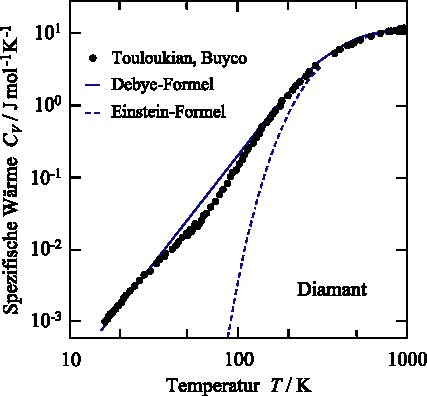
\includegraphics{Bilder/Debye_Einstein.pdf}
  \caption{Spezifische Wärme von Diamant in logarithmischer Darstellung~\cite{Hunklinger}. (Messwerte: Y.S. Touloukian, Thermophysical properties of Matter, Band V)}
  \label{fig:Debye_Einstein}
\end{figure}


%%%%%%% Gleichung mit einarbeiten %%%%%%%%%s
% \begin{align}\label{eqn:Waermeuebergangszahl}
%   \dot{Q} = \alpha \cdot A \cdot \Delta T, \quad \dot{q} = \alpha \Delta T.
% \end{align}


% *********************************************
% ***** KAPITEL 4 *****************************
% *********************************************
\newpage
\section{Ergebnisse und Diskussion}\label{sec:ErgebnisseUndDiskussion}

\subsection{Wahl der geeigneten Tieftemperaturmesstechnik}
Für die Messung tiefer Temperaturen ist die Wahl eines geeigneten Temperaturmessungsverfahren wichtig. Im Versuch werden zur Bestimmung der Temperatur Widerstandsthermometer wie Pt100 und Pt1000 verwendet. Dabei handelt es sich um Platinwiderstände, deren Widerstand bei \SI{273}{\kelvin} auf \SI{100}{\ohm} bzw. \SI{1000}{\ohm} liegt. Der Grund, warum Platin verwendet wird, liegt darin, dass es einerseits ein guter Wärmeleiter und ein edles Metall ist und andererseits in besonders reiner Form hergestellt werden kann, da sein Siedepunkt fern von denen anderer Metalle liegt.

\paragraph{Temperaturmessung mit Digitalmultimeter}$~$

Zu Beginn wird die Anfangstemperatur an den Platinwiderständen direkt mit der Temperatureinstellung des Digitalvoltmeters (DVM) gemessen, welche in Tabelle~\ref{tab:Temperaturmessung} dargestellt ist.

\begin{table}[htp]
    \centering
    \caption{Temperaturmessung der Raumtemperatur mithilfe von Pt100 und Pt1000 mithilfe eines Digitalmultimeters. Als Vergleich diente die Messung mit einem Quecksilberthermometer mit  $T = \SI{22.5\pm 0.2}{\celsius}$.}
    \label{tab:Temperaturmessung}
    \begin{tabular}{c S c}
      \toprule
      Widerstand & {Kompensation} & Temperatur \\
      \midrule
      Pt 100 & 0\,\si{\ohm} & \SI{35.1}{\celsius}\\
      & 4.9\,\si{\ohm} & \SI{22.4}{\celsius}\\
      Pt 1000 & 0\,\si{\ohm} & \SI{23.1}{\celsius}\\
      & 4.9\,\si{\ohm} & \SI{21.9}{\celsius}\\
      \bottomrule
    \end{tabular}
\end{table}

Es wurde jeweils eine Messung mit und ohne Kompensation des Leitungswiderstandes durchgeführt. Die Kompensation kann als Zahlenwert in das Multimeter eingegeben werden. Die Zuleitungswiderstände führen jeweils zur Hälfte hin und weg vom Platinwiderstand. Es ergab sich für den linken $R_1 = \SI{5.1}{\ohm}$ und $R_2 = \SI{4.7}{\ohm}$ für den rechten Zuleitungswiderstand. Für die Kompensation wurde der gemittelte Wert verwendet. Da die Vermessung der Leitungswiderstände für den Pt1000 Widerstand nicht möglich war, wurde hier der gleiche Widerstandswert angenommen. Tabelle~\ref{tab:Temperaturmessung} zeigt deutlich den Unterschied der Platinwiderstände ohne Kompensationsmessung. Für Pt100 ergibt sich ohne Leitungskompensation ein viel zu großer Temperaturwert, während der Zuleitungswiderstand beim Pt1000 ein prozentual geringeren Einfluss hat und das Ergebnis kaum verfälscht.

\begin{figure}[htp]
  \centering
  \begin{tikzpicture}
    \begin{axis}[disabledatascaling, width=0.98\textwidth, height=6cm, ylabel=Temperatur $T$ in \si{\kelvin}, xmin=0, xmax=120, xlabel={Widerstand $R$ in \si{\ohm}}]
      \addplot[mark=*,mark size=1pt,blue, thick] table[x index=0,y index=1]{Daten/Pt100_Kalibrierung.csv};
    \end{axis}
  \end{tikzpicture}
  \caption{Widerstandsabhängiger Temperaturverlauf des Pt100.}
  \label{fig:Pt100}
\end{figure}


Im weiteren Verlauf des Versuchs wird zur Temperaturmessung eine Konstantstromquelle verwendet und der temperaturabhängige Widerstand indirekt durch eine Spannungsmessung ermittelt. Zur Umrechnung der Widerstände in eine Temperatur wurde die Kalibrierungsdaten des Pt100 Sensors der Versuchsanleitung entnommen. Der Temperaturverlauf des Pt100 Sensors ist in Abbildung~\ref{fig:Pt100} dargestellt. Der Temperaturverlauf wurde zwischen den Literaturdaten interpoliert, damit beliebigen Widerständen im angegeben Bereich eine Temperatur zugeordnet werden kann.

\paragraph{Zweileiter- und Vierleiterschaltung}$~$

Für die Messung wurde eine regelbare Konstantstromquelle verwendet. Die Vermessung des Spannungsabfalls über den Widerstand erfolgt für beide Platinwiderstände jeweils in Zweileiter- und Vierleiterschaltung für drei verschiedene Ströme. Die Ergebnisse sind in Tabelle~\ref{tab:Zwei_Vierleiterschaltung} dargestellt.

\begin{table}[htp]
    \centering
    \caption{Bestimmung der Raumtemperatur durch Spannungsmessung mit dem Digitalmultimeter in Zweileiter- und Vierleiterschaltung für verschiedene Ströme.}
    \label{tab:Zwei_Vierleiterschaltung}
    \begin{tabular}{c c r S S S S}
      \toprule
      Widerstand & Schaltung & {$I$ [\si{\micro\ampere}]} & {$U$ [\si{\milli\volt}]} & {$R$ [\si{\ohm}]} & {$T$ [\si{\kelvin}]} & $\vartheta$ [\si{\celsius}]\\
      \midrule
      Pt 100 & Zweileiter & 100 & 11.328 & 113.33 & 307.4 & 34.3 \\
       & & 10 & 1.130 & 113.00 & 306.6 & 33.4 \\
       & & 5 & 0.567 & 113.40 & 307.6 & 34.5 \\
      & Vierleiter & 100 & 10.862 & 108.86 & 295.9 & 22.8 \\
      & & 10 & 1.084 & 108.40 & 294.7 & 21.6 \\
      & & 5 & 0.545 & 109.00 & 296.3 & 23.1\\
      \midrule
      Pt 1000 & Zweileiter & 100 & 108.621 & 108.62 & 295.2 & 22.1 \\
      & & 10 & 10.8 & 108.00 & 293.7 & 20.5 \\
      & & 5 & 5.402 & 108.04 & 293.7 & 20.5 \\
      \bottomrule
    \end{tabular}
\end{table}

Es zeigt sich auch hier, dass die gemessene Temperatur des Pt 100 in Zweileiterschaltung zu groß ist, was durch endlichen Leitungswiderstände hervorgerufen wird. Wird die Schaltung jedoch als Vierleiterschaltung aufgebaut, kann das Problem der Leitungswiderstände umgangen werden. Einen Vergleich von Zwei- und Vierleiterschaltung zeigt Abbildung~\ref{fig:Schaltung}

\begin{figure}[htp]
  \centering
  \begin{tikzpicture}
    \draw (0,0) to[current source] (3,0) to (3,3) to[R=$R$] (0,3) to (0,0);
    \draw (0,1.5)node[circ]{} to (1.5,1.5)node[draw,circle,fill=white] {V} to (3,1.5)node[circ]{};
    \node (A) at (1.5,-.7){Zweileiterschaltung};
    \begin{scope}[shift={(6,0)}]
      \draw (0,0) to[current source] (3,0) to (3,3) to[R=$R$] (0,3) to (0,0);
      \draw (0.7,3)node[circ]{} to(0.7,1.5) to (1.5,1.5)node[draw,circle,fill=white] {V} to (2.3,1.5) to (2.3,3)node[circ]{};
      \node (A) at (1.5,-.7){Vierleiterschaltung};
    \end{scope}
  \end{tikzpicture}
  \caption{Zwei- und Vierleiterschaltung im Vergleich. Da die Abstände von den Messgeräten zu den Temperaturwiderständen in der Regel groß sind, sind Leitungswiderstände nicht vernachlässigbar. Bei der Vierleiterschaltung wird ein zusätzliches Leitungspaar verlegt, welches die Spannung kurz vor und hinter dem Widerstand abgreift. Aufgrund des viel größeren Widerstandes des Voltmeters gegenüber der Stromquelle, fließt in diesem Stromkreis fast kein Strom, was nahezu kein Spannungsabfall über der Leitung ergibt.}
  \label{fig:Schaltung}
\end{figure}


Für den Pt 1000 Widerstand konnte aufgrund des Aufbaus keine Messung in Vierleiterschaltung durchgeführt werden. Allerdings sind hier die Auswirkungen des Leitungswiderstandes um das zehnfache geringer. Es zeigt sich, dass eine große Temperaturauflösung durch die Wahl eines größeren Stromes erzielt werden kann, da hierbei eine kleinere Spannungsänderung noch durch das Digitalmultimeter aufgelöst werden kann. Jedoch steigt die Heizleistung $P = I R^2$ linear mit der Stromstärke an. Für hohe Stromstärken heizt sich der Temperaturfühler auf und gerät mit der zu messenden Probe aus dem thermischen Gleichgewicht. Die Messung wird verfälscht.

Zur Bestimmung des optimalen Stroms der Konstantstromquelle wird zunächst eine Überlegung durchgeführt, welche Temperaturauflösung gewünscht ist. Für die Messung wurde eine Auflösung von $\Delta T = \SI{0.1}{\kelvin}$ angepeilt. Ein Vergleich mit den Kalibrierungsdaten zeigt, dass der lineare Anstieg des Widerstandes
\begin{align}
  \frac{(100.72-98.76)\si{\ohm}}{(275-270)\si{\kelvin}} = \SI{0.392}{\ohm\per\kelvin}
\end{align}
entspricht. Für die gewünschte Temperaturauflösung ist somit eine Widerstandsauflösung von $\Delta R = \SI{0.04}{\ohm}$ nötig. Mit einer Spannungsauflösung des Multimeters von $\Delta U = \SI{1}{\micro\volt}$ ergibt sich ein Strom von
\begin{align}
  I = \frac{\Delta U}{\Delta R} = \SI{25}{\micro\ampere}.
\end{align}

\paragraph{Temperaturmessung mit Siliziumdiode}$~$

Zur Messung des temperaturabhängigen Widerstandes einer Siliziumdiode wurde eine separate Gleichstromquelle mit $I = \SI{10}{\micro\ampere}$ verwendet. Die Kalibrierungsdaten der Temperatur als Funktion der Spannung sind in Abbildung~\ref{fig:Diode} dargestellt.

\begin{figure}[htp]
  \centering
  \begin{tikzpicture}
    \begin{axis}[disabledatascaling, width=\textwidth, height=6cm, ylabel=Temperatur $T$ in \si{\kelvin}, xmin=0.1, xmax=1.7, xlabel={Spannung $U$ in \si{\volt}}]
      \addplot[mark=*,mark size=1pt,blue, thick] file[x index=1,y index=2]{Daten/Kalibrierung_Diode.csv};
    \end{axis}
  \end{tikzpicture}
  \caption{Spannungsabhängiger Temperaturverlauf der Siliziumdiode.}
  \label{fig:Diode}
\end{figure}


Bei der Messung ergaben sich die in Tabelle~\ref{tab:Diode} dargestellten Ergebnisse.
\begin{table}[htp]
    \centering
    \caption{Spannungsmessung an einer Siliziumdiode bei Raumtemperatur mithilfe eines Digitalmultimeters mit einer Messgenauigkeit von \SI{10}{\micro\volt}. Als Vergleich diente die Messung mit einem Quecksilberthermometer mit  $T = \SI{22.5\pm 0.2}{\celsius}$.}
    \label{tab:Diode}
    \begin{tabular}{c S S S}
      \toprule
      Schaltung & {$U$ [\si{\milli\volt}]} & {$T$ [\si{\kelvin}]} & $\vartheta$ [\si{\celsius}] \\
      \midrule
      Zweileiter & 0.52918 & 295.73 \pm 0.01 & 22.58 \pm 0.01 \\
      Vierleiter & 0.52916 & 295.74 \pm 0.01 & 22.59 \pm 0.01 \\
      \bottomrule
    \end{tabular}
\end{table}

Es zeigt sich, dass die Messwerte für beide Schaltungstypen beinahe identisch sind, was sich durch den großen Widerstand der Diode erklären lässt. Bei Raumtemperatur beträgt dieser
\begin{align}
  R = \frac{U}{I} = \frac{\SI{0.52918}{\volt}}{\SI{10}{\micro\ampere}} = \SI{52.92}{\kilo\ohm}.
\end{align}

\newpage
\subsection{Bandlückenbestimmung eines dotierten Halbleiters}

\begin{wrapfigure}{r}{6cm}
  \vspace{-.5cm}
  \centering
  \begin{tikzpicture}
    \begin{axis}[width=6cm, height=6cm, xlabel=Zeit $t$ in \si{\minute}, xmin=100, xmax=140, ymin=110, ymax=160, ylabel={$T$ in \si{\kelvin}}, legend cell align={left}, xtick scale label code/.code={}]
      \addplot[blue] table[x index=0,y index=1]{Daten/Halbleitermessung_Zeitverlauf.txt};
      \addplot[orange ] table[x index=0,y index=2]{Daten/Halbleitermessung_Zeitverlauf.txt};
      \addplot[green!50!black] table[x index=0,y index=3]{Daten/Halbleitermessung_Zeitverlauf.txt};
      \legend{Pt 100, Pt 1000, Diode};
    \end{axis}
  \end{tikzpicture}
  \caption{Temperaturkurven der Mess\-widerstände}
  \label{fig:Temperaturvergleich}
\end{wrapfigure}


In diesem Versuchsteil wurde der temperaturabhängige Widerstand eines golddotierten Germaniumhalbleiters untersucht. Dieser weist, wie in Abschnitt~\ref{sec:Widerstand} erläutert, eine exponentielle Abhängigkeit von der Temperatur auf. Der Halbleiter wurde in einem Zeitraum von \SI{2.5}{\hour} kontinuierlich mithilfe einer Gifford-McMahon Kleinkältemaschine von Zimmertemperatur auf \SI{80}{\kelvin} abgekühlt. Zur Aufzeichnung der Temperatur wurden ein Pt 100 Widerstand in Vierleiterschaltung, ein Pt 1000 Widerstand in Zweileiterschaltung und eine Siliziumdiode verwendet. Für die Datenauswertung wurde die Diode verwendet, da aufgrund der großen Änderung des Widerstands bei kryogenen Temperaturen die Temperaturbestimmung am genauesten erfolgt. Ein Vergleich der drei Temperaturbestimmungsarten in Abbildung~\ref{fig:Temperaturvergleich} zeigt jedoch, dass alle drei Widerstandsthermometer fast identische Temperaturwerte liefern, die sich maximal um \SI{\pm1}{\kelvin} unterscheiden.

Die aufgenommenen Spannungswerte wurden mithilfe der in der Versuchsanleitung~\cite{Thurk} gegebenen Kalibrierungstabelle (siehe Abbildung~\ref{fig:Diode}) in Temperaturen umgerechnet. Als Referenzwiderstand wurde $R_0 = \SI{1}{\ohm}$ gewählt.

\begin{figure}[htp]
  \centering
  \begin{tikzpicture}
    \begin{axis}[disabledatascaling, width=\textwidth, height=6cm, ylabel=Absorptionsrate, xlabel=Wellenlänge $\lambda$ in \si{\nano\metre}, xmin = 950, xmax=2150, xtick={}, ymin =-.1, ymax = 1.15, legend cell align={left}]
      \filldraw[draw=white!80!orange,fill=white!90!orange] (1020,-.1) rectangle (1080,1.2);
      \draw[thick, white!50!orange] (1050,-.1) -- (1050,1.2);
      \filldraw[draw=green!50!black, draw opacity = 0.2,fill=green!50!black, fill opacity = 0.1] (1770,-.1) rectangle (1830,1.2);
      \draw[thick, green!50!black, opacity = 0.5] (1800,-.1) -- (1800,1.2);
      \addplot[orange, thick] file[x index=1,y index=2]{Daten/Absorption_Smooth_Kalibrierung_Glasprisma_Wolframlampe5V_kleinesHalbleiterplaettchen_3_6Grad_500nm_all100nmMaker_Spalt_500mu.txt};
      \addlegendentry{Silizium}
      \addplot[green!50!black, thick] file[x index=1,y index=2]{Daten/Absorption_Smooth_Kalibrierung_Glasprisma_Wolframlampe5V_mitgrossemHalbleiterplaettchen_3_6Grad_500-3200nm_mitMarkern2_Spalt_500mu.txt};
      \addlegendentry{Germanium}
    \end{axis}
  \end{tikzpicture}
  \caption{Transmissionsrate von Silizium und Germanium.}
  \label{fig:Halbleitermessung_relativ}
\end{figure}


Die Größe der Bandlücke lässt sich nun mithilfe von Gleichung~\eqref{eqn:Anstieg_Bandlücke} bestimmen. Dafür wird wird der natürliche Logarithmus $\ln(R_0/R)$ über die inverse Temperatur $1/T$ aufgetragen und eine lineare Funktion an die Messdaten angefittet, wie in Abbildung~\ref{fig:Halbleitermessung} dargestellt ist. Es ergibt sich nun für eine lineare Fitfunktion der Form $y(x) = a + b\cdot x$
\begin{align}
  \ln\qty(\frac{R_0}{R}) = - \frac{\Delta E}{k_B}\frac{1}{T} \quad \Rightarrow \quad \Delta E = - b \cdot k_B.
\end{align}
Der lineare Anstieg, kann aus dem Fit abgelesen werden und es ergibt sich
\begin{align}
  \Delta E = -\SI{-1698.3\pm 1.3}{\kelvin} \cdot k_B = \SI{0.1463\pm0.0001}{\electronvolt}.
\end{align}
Da die Dotierung des Germaniums nicht genau bekannt ist, kann dieser Wert nicht mit der Literatur verglichen werden. Es lässt sich nur die Abschätzung treffen, dass die Bandlücke des dotierten Halbleiters unterhalb der von reinem Germanium liegt, welche bei $T=\SI{300}{\kelvin}$ die Größe $E_g = \SI{0.66}{\electronvolt}$ hat~\cite{Hunklinger}. Die ermittelte Bandlücke ist nur ein fünftel von der des reinen Germaniums. Dies lässt sich dadurch erklären, dass im Mangelhalbleiter das Akzeptorniveau knapp oberhalb des Valenzbandes liegt und Elektronen schon bei geringeren Energien in das Leitungsband gelangen können.

\subsection{Abkühlverhalten kryogener Flüssigkeiten}

Dieser Abschnitt beschäftigt sich mit dem Abkühlverhalten eines Kupferzylinders, welcher in flüssigen Stickstoff getaucht wird. Der zylindrische Probenkörper enthält in der Mitte einen Pt~100 Widerstand, der als Temperaturfühler dient. Zur Messung der Temperatur, wird der Pt~100 an eine Stromversorgung angeschlossen, bei welcher der Strom so eingestellt wurde, dass der Spannungsabfall über den Widerstand den Wert \SI{10}{\volt} nicht übersteigt, weil der Analog-Digital-Wandler zur PC gestützen Aufnahme der Daten nur maximal diese Spannung akzeptiert. Da die Messung bei Raumtemperatur startet, wurde an der Stromquelle ein Wert von $I = \SI{68.46}{\milli\ampere}$ eingestellt. Das aufgenommene Spannungssignal kann damit in einen Widerstand und anschließend eine Temperatur umgerechnet werden.

Die Abkühlung des Probenkörpers erfolgte auf zwei verschiedene Arten und Weisen. Zunächst wurde der Probenkörper ohne Isolierung in den Stickstoff getaucht und anschließend ein zweiter, identischer Probenkörper mit einer aus Papier bestehenden Isolierung. Die aufgenommenen Temperaturverläufe sind in Abbildung~\ref{fig:Abkuehlung} dargestellt.

\begin{figure}[htp]
  \centering
  \begin{tikzpicture}
    \begin{axis}[disabledatascaling, width=.95\textwidth, height=6cm, ylabel=Temperatur $T$ in \si{\kelvin}, xmin=0, xmax=300, ymin=50, xlabel={Zeit $t$ in \si{\second}}, legend cell align={left}]
      \fill[fill=blue!50!black, opacity = 0.05] (10,0) rectangle (241,350);
      \fill[fill=green!50!black, opacity = 0.05] (300,0) rectangle (250,350);
      \addplot[blue, thick] file[x index=1,y index=2]{Daten/Kalibrierung_Pt100_abkuehlung_Widerstand.txt};
      \addlegendentry{ohne Isolierung}
      \addplot[orange, thick] file[x index=1,y index=2]{Daten/Kalibrierung_Pt100_Isolierung_Widerstand.txt};
      \addlegendentry{mit Isolierung}
      \draw[dotted] (0,77.35) -- +(290,0);
      \node at (30,84){\SI{77.4}{\kelvin}};
      \draw[dashed, green!50!black] (241,0) -- +(0,300);
      \draw[dashed, green!50!black] (250,0) -- +(0,300);
      \node[anchor=east]at (241,175) {\small Filmsieden};
      \node[anchor=west]at (250,175) {\small Blasensieden};
      % \addplot[red, thick, domain=246:254]{757.525-2.61864*x};
      % \addplot[red, thick, domain=251:261]{457.12515-1.43091*x};
      \addplot[red, thick, domain=262:278]{178.3379-0.36135*x};
      \addlegendentry{Lineare Anpassung}
      \addplot[red, thick, domain=183:238]{259.41293-0.57618*x};
      \fill[red!50!black] (211,138) circle(1pt)node[below left]{\small\SI{138}{\kelvin}};
      % \fill[red!50!black] (250,102) circle(1pt)node[above right]{\small\SI{102}{\kelvin}};
      % \fill[red!50!black] (256,90) circle(1pt)node[above right]{\small\SI{90}{\kelvin}};
      \fill[red!50!black] (270,80.58) circle(1pt)node[above right]{\small\SI{80.5}{\kelvin}};
    \end{axis}
  \end{tikzpicture}
  \caption{Zeitlicher Temperaturverlauf eines Kupferzylinders beim Eintauchen in flüssigen Stickstoff. Es sind zudem die Bereiche des Film und Blasensiedens eingezeichnet. Dazwischen liegt ein Übergangsgebiet mit einer stark ansteigenden Wärmestromdichte. Für beide Siedevorgänge wurde mithilfe einer linearen Anpassung der Temperaturgradient bestimmt.}
  \label{fig:Abkuehlung}
\end{figure}


Der Temperaturverlauf des Probenkörpers mit Isolierung zeigt, dass der eingestellte Strom zu groß gewählt wurde, weil sich zu Beginn der Datenaufnahme (die Messung beginnt erst bei $t= \SI{25}{\second}$) die Probe auf über \SI{300}{\kelvin} erwärmt. Die Platinwiderstand wird also durch den Stromfluss erwärmt und verfälscht die Messung, der qualitative Verlauf bleibt jedoch trotzdem erhalten.

Es zeigt sich, dass sich der Probenkörper mit Isolierschicht schneller abkühlt als der Kupferzylinder ohne Isoliermaterial. Trotz der isolierenden Wirkung des Papiermantels verläuft die Wärmeübertragung schneller. Diese zunächst widersprüchliche erscheinende Beobachtung lässt sich mithilfe des \textsc{Leidenfrost}'schen Phänomens und dem damit verbundenen Filmsieden erklären. Ohne Papierschicht bildet sich auf der Oberfläche des Kupferzylinders aufgrund des großen Temperaturgefälles ein Gasfilm aus Stickstoff aus, der eine höhere isolierende Wirkung als das Papier aufweist, weshalb dieser Siedevorgang als Filmsieden bezeichnet wird. Der Wärmeübergangskoeffizient $\alpha$ liegt beim Filmsieden wesentlich niedriger als beim Blasensieden, wo ein direkter Kontakt der Flüssigkeit besteht, da beim Filmsieden der Wärmetransport hauptsächlich durch Strahlung anstatt durch Konvektion erfolgt. Der Grund, warum sich auf dem Papier kein Gasfilm ausbildet, liegt in der schlechten Wärmeleitfähigkeit des Papiers. Hier ergibt sich zwischen Papierinnenseite und -oberfläche ein großer Temperaturgradient. Die Temperatur auf der Papieroberfläche ist damit gering genug, damit das Filmsieden ausbleibt und direkt das Blasensieden (siehe Abschnitt~\ref{sec:Sieden}) einsetzt.

Experimentell lässt sich der Umschlag zwischen Film- und Blasensieden nach \SI{140}{\second} nach Eintauchen des Probenkörpers beobachten, weil dort eine stark erhöhte Blasenbildung auftritt, da hier die Wärmestromdichte und somit die Menge des verdampften Stickstoffs besonders hoch ist.

Für den Kupferzylinder mit Papierisolierung lässt sich keine Wärmeübergangszahl bestimmen, da aufgrund des großen Temperaturgradienten keine homogene Temperaturverteilung zustande kommt. Stattdessen finden zwei Wärmeübergänge statt, vom Kupfer zum Papier und anschließend zum Stickstoff.

\subsubsection{Bestimmung der Wärmeübergangszahl}

Zur Bestimmung der Wärmeübergangszahl nach~\eqref{eqn:Waermeuebergangszahl} muss zunächst die Heizleistung $\dot{Q}$ bestimmt werden. Diese ergibt sich nach dem ersten Hauptsatz der Thermodynamik zu
\begin{align}\label{eqn:Heizleistung}
  \dot{Q} = m_\text{Cu} C_\text{Cu} \dv{T}{t},
\end{align}
wobei $C_\text{Cu}$ die spezifische Wärmekapazität und $m_\text{Cu}$ die Masse von Kupfer bezeichnen. Der Temperaturgradient lässt sich aus dem Anstieg der Temperaturkurve in Abbildung~\ref{fig:Abkuehlung} gewinnen durch eine lineare Anpassung. Für das Film- und Blasensieden ergibt
\begin{align}
  \dv{T}{t} &= \SI{-0.3614\pm 0.0055}{\kelvin\per\second} \quad (\text{Blasensieden})\\
  \dv{T}{t} &= \SI{-0.5762\pm 0.0004}{\kelvin\per\second} \quad (\text{Filmsieden}).
\end{align}
Die Masse des Kupferzylinders kann mithilfe des Volumens und der Dichte $\varrho = \SI[per-mode=symbol]{8960}{\kilo\gram\per\metre\cubed}$~\cite{Fastowski} von Kupfer bestimmt werden. Mit einem Durchmesser $d = \SI{3 \pm 0.05}{\centi\metre}$ und einer Höhe von $h=\SI{8.5\pm 0.05}{\centi\metre}$ ergibt sich eine Masse von
\begin{align}
  m = \varrho \cdot V = \varrho \frac{\pi d^2}{4}h = \SI{0.359\pm 0.021}{\kilo\gram}.
\end{align}
Ein Vergleich von~\eqref{eqn:Waermeuebergangszahl} mit~\eqref{eqn:Heizleistung} ergibt sich
\begin{align}\label{eqn:alpha}
  \alpha = \frac{\dot{Q}}{A (T_\text{\ce{N2}}-T_\text{Cu})} = \frac{m_\text{Cu} C_\text{Cu} \dv{T}{t}}{A (T_\text{\ce{N2}}-T_\text{Cu})}.
\end{align}
Die Oberfläche des Zylinders ergibt sich zu $A = \SI{94.3\pm5.3}{\centi\metre\squared}$.

Die spezifische Wärmekapazität von Kupfer wurde an einem ausgewählten Punkt jeweils fürs Film- und Blasensieden berechnet (siehe Abbildung~\ref{fig:Abkuehlung}). Dabei wird eine Tabelle aus~\cite[S.353]{Fastowski} für die spezifische Wärme in Abhängigkeit von $\Theta/T$ genutzt. Die spezifische Wärmekapazität bei den beiden Temperaturen zeigt Tabelle~\ref{tab:Waermekapazität_Kupfer}.
\begin{table}[htp]
  \centering
  \caption{Bestimmung der Wärmekapazität des Kupfers bei verschiedenen Temperaturen. Zur Umrechnung in die masseabhängige Wärmekapazität wurde durch die molare Masse von Kupfer $M_\text{Cu} = \SI{63.55}{\gram\per\mol}$ geteilt.}
  \label{tab:Waermekapazität_Kupfer}
  \begin{tabular}{c c c c}
    \toprule
    & $T$ [\si{\kelvin}] & $C_V$ [\si{\calorie\per\mole\per\kelvin}] & $C_V$ [\si{\joule\per\kilo\gram\per\kelvin}]\\
    \midrule
    Filmsieden & 138 & 4.74 & 312.1  \\
    Blasensieden & 80.5 & 3.18 & 209.4 \\
    \bottomrule
  \end{tabular}
\end{table}

Mithilfe des Siedepunkts von Stickstoff bei $T_\text{\ce{N2}} = \SI{77.4}{\kelvin}$ ergibt sich für die Wärmeübergangszahl $\alpha$ nach~\eqref{eqn:alpha}
\begin{align}
  \alpha_\text{FS,exp.} &= %\frac{-0.359\cdot 312.1\cdot \SI{0.5762}{\watt}}{\SI{8.8e-3}{\metre\squared}(77.4-138)\si{\kelvin}} =
  \SI{112\pm 17}{\watt\per\square\metre\per\kelvin}\\
  \alpha_\text{BS,exp.} &= %\frac{-0.359\cdot 209.4\cdot \SI{0.3614}{\watt}}{\SI{8.8e-3}{\metre\squared}(77.4-80.5)\si{\kelvin}} =
  \SI{930\pm 150}{\watt\per\square\metre\per\kelvin}
\end{align}
Die großen Fehlerbereiche ergeben sich aufgrund der nur recht ungenau bestimmbaren Masse des Kupferzylinders und der Oberfläche. Weitere mögliche Fehler durch die Wärmekapazität wurden nicht berücksichtigt. Es wurde zudem die Annahme getroffen, dass der Zylinder vollständig aus Kupfer besteht, jedoch befindet sich innerhalb noch der Pt 100 Widerstand.

Mit der Literatur~\cite{Fastowski} lässt sich eine Vergleichsrechnung durchführen. Ein Vergleich mit Abbildung~\ref{fig:Sieden_Stickstoff} ergibt einen Ausdruck für die Wärmestromdichte für das Film- und Blasensieden.
\begin{figure}[htp]
  \centering
  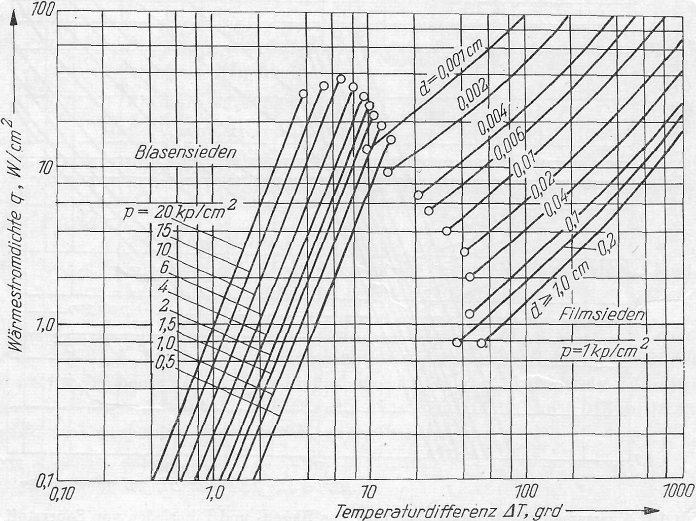
\includegraphics[width=0.7\textwidth]{Bilder/Sieden_Stickstoff.pdf}
  \caption{Zusammengefasste Ergebnisse des Blasen- und Filmsiedens von Stickstoff im großen Volumen ($d=$ Durchmesser des Heizers)~\cite[S.230]{Fastowski}.}
  \label{fig:Sieden_Stickstoff}
\end{figure}

Für das Filmsieden ergibt sich mit $d = \SI{3}{\centi\metre} > \SI{1}{\centi\metre}$ und einer Temperaturdifferenz von  \SI{60\pm 1}{\kelvin} eine Wärmestromdichte von $\dot{q} = \SI[per-mode=symbol]{0.85\pm 0.05}{\watt\per\centi\metre\squared}$. Für das Blasensieden ergibt sich bei Normaldruck\footnote{Das Kilopond ist eine veraltete Einheit der Kraft. $\SI{1}{\kilo\text{p}} = \SI{9.807}{\newton}$}. $p \approx \SI{1}{\kilo\text{p}\per\centi\metre\squared}$ und einer Temperaturdifferenz von \SI{3\pm 0.2}{\kelvin} eine Wärmestromstromdichte von $\dot{q}= \SI{0.3 \pm 0.05}{\watt\per\centi\metre\squared}$. Somit lässt sich nach~\eqref{eqn:Waermeuebergangszahl} die Wärmeübergangszahl schreiben als
\begin{align}
  \alpha_\text{FS,Theorie} &=
  \SI{141\pm 10}{\watt\per\square\metre\per\kelvin}\\
  \alpha_\text{BS,Theorie} &=
  \SI{1000\pm 170}{\watt\per\square\metre\per\kelvin}.
\end{align}

\subsubsection{Wärmeübergangszahl des Filmsiedens nach der Ähnlichkeitstheorie}

Die Wärmeübertragung beim Filmsieden erfolgt ebenfalls durch Strahlung. Dabei lässt sich das Filmsieden eines verflüssigten Gases an der äußeren Oberfläche eines horizontalen Zylinders durch folgende Gleichung beschreiben~\cite{Fastowski}:
\begin{align}\label{eqn:Filmsieden_Theorie}
  \frac{\alpha d}{\lambda_m} = 0.62 \qty[\frac{d^3 \varrho_m(\varrho_\text{fl}-\varrho_m)g \cdot l_d}{\lambda_m \eta_m \Delta T}\qty(1+0.4\frac{c_{p,m}\Delta T}{l_d})^2]^{\frac{1}{4}}.
\end{align}
Für den Temperaturunterschied wurde $\Delta T = (138-77.4)\si{kelvin} = \SI{60.6}{\kelvin}$ angenommen. Die weiteren  von Stickstoff erforderlichen Größen sind mit der Fallbeschleunigung in Tabelle~\ref{tab:Groessen} zusammengefasst.
\begin{table}[htp]
  \centering
  \caption{Größen für die Bestimmung der Wärmeübergangszahl. Der Index $m$ weist darauf hin, dass für die charakteristischen Größen des Gases die mittlere Temperatur $\frac{1}{2}(T_\text{Cu}+T_\text{\ce{N2}}) = \SI{107.7}{\kelvin}$ verwendet wird.}
  \label{tab:Groessen}
  \begin{tabular}{l l l c}
    \toprule
    Größe & & Wert & Quelle \\
    \midrule
    Dichte von \ce{N2(g)} & $\varrho_m$ & \SI{3.24}{\kilo\gram\per\metre\cubed} & \cite{Wolfram}\\
    Dichte von \ce{N2(l)} & $\varrho_{fl}$ & \SI{810.6}{\kilo\gram\per\metre\cubed} & \cite{Wolfram}\\
    Wärmeleitfähigkeit von \ce{N2(g)} & $\lambda_m$ &\SI{10.1e-3}{\watt\per\metre\per\kelvin} & \cite{Wolfram}\\
    Dynamische Viskosität von \ce{N2(g)} & $\eta_m$ & \SI{7.48e-6}{\kilo\gram\per\metre\per\second} & \cite{Wolfram}\\
    Verdampfungswärme \ce{N2} & $l_d$ & \SI{47.073}{\calorie\per\gram} & \cite{Fastowski}\\
    Fallbeschleunigung & $g$ & \SI{9.81}{\metre\per\second\squared} & \\
    Spezifische Wärme \ce{N2(g)} & $c_{p,m}$ & \SI{1064}{\joule\per\kilo\gram\per\kelvin} & \cite{Wolfram}\\
    \bottomrule
  \end{tabular}
\end{table}
Werden alle Größe in Gleichung~\eqref{eqn:Filmsieden_Theorie} eingesetzt, ergibt sich umgestellt nach der Wärmeübergangszahl $\alpha$
\begin{align}
  \alpha = \SI{92.3\pm 4.5}{\watt\per\metre\squared\per\kelvin}.
\end{align}
Zur Fehlerabschätzung wurden nur mögliche Fehler der Temperaturmessung $\Delta T$ und Durchmesserbestimmung beachtet und die Größen in Tabelle~\ref{tab:Groessen} als fehlerlos angenommen. Es zeigt sich, dass der Messwert für die Übergangszahl des Filmsiedens zwischen den berechneten Werten nach dem ähnlichen Modell und Abbildung~\ref{fig:Sieden_Stickstoff} liegt. Allerdings lässt sich durch das Modell das reale Experiment nicht vollständig beschreiben, da ebenfalls der Einfluss der Befestigungsstab vernachlässigt wird und von einem idealen Kupferzylinder ausgegangen wird.
% *********************************************
% ***** KAPITEL 5 *****************************
% *********************************************
\newpage
\section{Zusammenfassung}

% ***** Literaturverzeichnis ******************

\bibliography{Literatur}{}
\bibliographystyle{plain}
\end{document}
